\documentclass{article}
\usepackage{blindtext}
\usepackage{cite}
\usepackage{float}
\usepackage{tabu}
\usepackage{subcaption}
\usepackage{graphicx}


\begin{document}

\begin{titlepage}
	\centering
	{\huge\bfseries Title \par}
	\vspace{2cm}
	Simon Willimann

	\vfill
	\begin{flushleft}
	University of Zurich\\
	04.11.2021
	\end{flushleft}



%\title{Title}
%\author{Simon Willimann}
%\date{04.11.2021}

\end{titlepage}



\begin{abstract}
abstract yada yada

\end{abstract}
\newpage

\section*{Thanks}
To you, Igor, and my teammates, Shujun and Wenying.

\section{Main}
\Blindtext[7]
blabla\cite{Gormsen2020} \\
blablabla\cite{Kozlowski2020}


\begin{figure}
		\centering
		\makebox[\textwidth][c]{  
		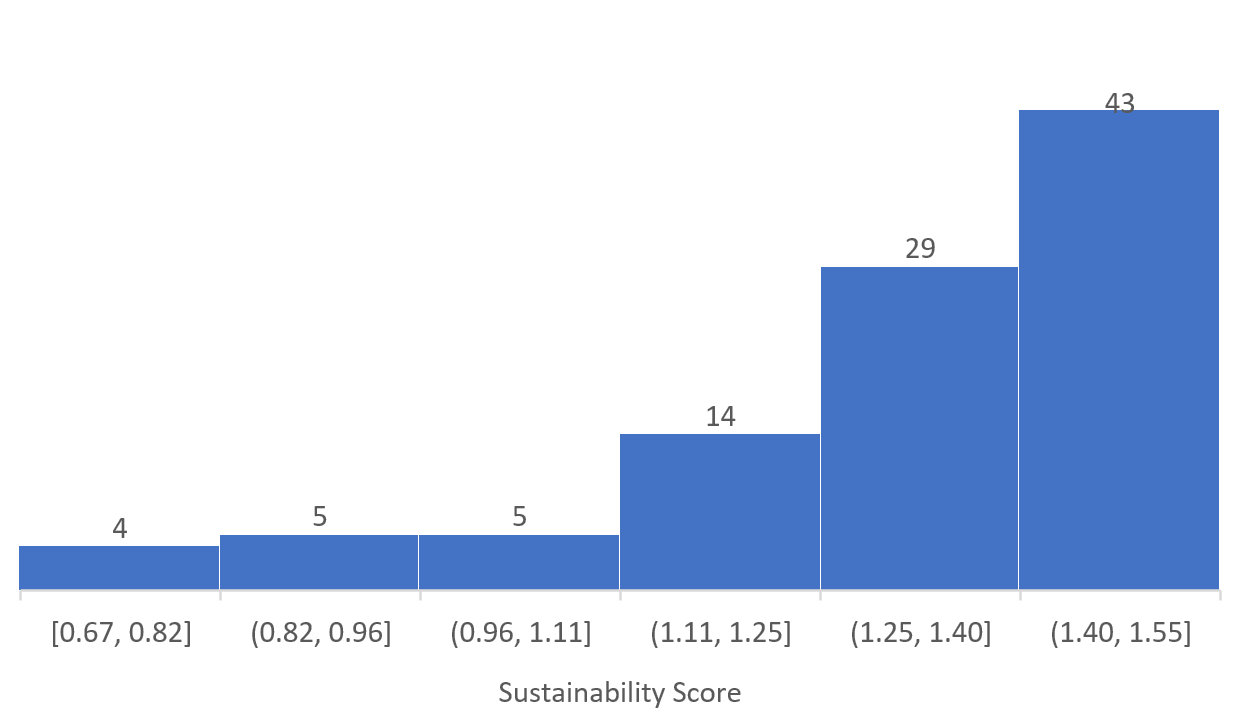
\includegraphics[width=0.8\linewidth]{DISTSUS.png}}
  		\caption{}
        \emph{Distribution of Sustainability Scores}
\end{figure}

\begin{figure}


	\makebox[\textwidth][c]{
    \begin{tabu}{c c c c c}
    \hline
        \rowfont[c]{\bfseries}Company & Country & Market Cap & Revenue & SS \\ \hline\hline
        Nomad Foods & UK & 4,376.80 & 800 & 1.5468 \\ 
        Mitsubishi Corporation & Japan & 31,561.73 & 3400 & 1.5158 \\ 
        Mowi & Norway & 11,487.50 & 3694 & 1.4712 \\ 
        Charoen Pokphand Foods & Thailand & 6,959.73 & 1917 & 1.2697 \\ 
        Thai Union Group & Thailand & 2,163.60 & 3752 & 1.0533 \\ 
        Nippon Suisan Kaisha (Nissui) & Japan & 1,379.90 & 5707 & 0.7859 \\ 
        High Liner Foods & Canada & 290.48 & 956 & 0.7739 \\ 
        Maruha Nichiro & Japan & 1,102.50 & 7158 & 0.7618 \\ 
        Marubeni Corporation & Japan & 8,680.24 & 1900 & 0.7223 \\ 
        Kyokuyo & Japan & 253.62 & 2123 & 0.6924 \\ 
        SalMar & Norway & 6,631.40 & 1044 & 0.5449 \\ 
        Austevoll Seafood ASA & Norway & 2,070.47 & 2186 & 0.5262 \\ 
        Yokohama Reito (Yokorei) & Japan & 508.50 & 940 & 0.2835 \\ 
    \end{tabu}}
    \caption{}
    \centering
    \emph{Companies and their Sustainability Score}
\end{figure}


\newpage

\bibliographystyle{plain}
\bibliography{citations.bib}




\end{document}

